%% Copyright (C) 2012, Gostai S.A.S.
%%
%% This software is provided "as is" without warranty of any kind,
%% either expressed or implied, including but not limited to the
%% implied warranties of fitness for a particular purpose.
%%
%% See the LICENSE file for more information.

\chapter{Getting started}

\section{Documentation and Support}

\subsection{Jazz User Manual}

Jazz User Manual contains all the information needed to set up your robot,
and daily use it: control it with its joystick, control it remotely through
Internet (Jazz Connect), set up watch for your premises and configure alerts
(Jazz Security), or launch special behaviors (Jazz Connect).

\ifthen{\NOT\boolean{urbisdk}}
{
  \subsection{Open Jazz Developer Manual}

  This documentation extends the Urbi SDK documentation, and describe the
  Urbi programming API for the Jazz robot. We recommend that you be familiar
  with the Urbi SDK before reading this documentation.

  \subsection{Urbi SDK}

  The Urbi SDK is a fully-featured environment to orchestrate complex
  organizations of components. It relies on a middleware architecture that
  coordinates components named UObjects. It also features \us, a scripting
  language that can be used to write orchestration programs. If you are not
  familiar with the Urbi robotic software development platform, we recommend
  that you first read the Urbi SDK documentation:
  \url{http://gostai.com/support/documentation/}.

  With the Urbi documentation you need to understand:
  \begin{itemize}
  \item the overall Urbi architecture, with \us language and UObject
    components
  \item how to program using \us
  \item how to extend Urbi writing UObjects, and how to use your UObjects
    from \us
  \end{itemize}
}

\subsection{Getting Support}

Gostai provides commercial support and services, in the form of support
packs that you can purchase
(\url{http://gostai.com/support/support_packs/}).  Gostai experts can help
you master the Jazz SDK, and assist you with your with Jazz development.  To
contact Gostai support: \email{support@gostai.com}.

\section{Requirements}

In order to communicate with, and program Jazz, you need
\begin{itemize}
\item a Local Area Network (LAN) with DHCP.
\item a WiFi access point to your LAN. ESSID \strong{must not} be hidden.
\item a computer connected to your LAN with at least
  \begin{itemize}
  \item 1.5 GHz CPU
  \item 512 MB RAM
  \item WiFi card (for wireless connection between computer and Jazz
    in ad-hoc mode)
  \item Mac OS X Snow Leopard 10.6, GNU/Linux 32 bits, Windows XP 32 bits
  \item \usdk 2.7.3
  \item ssh client (\command{putty} on Windows, \command{ssh} on GNU/Linux
    or Mac OS X)
  \item scp client (\command{pscp} or \command{WinSCP} on windows,
        \command{scp} on GNU/Linux or Mac OS X)
  \item telnet client (Gostai Lab, Gostai Console, GNU Netcat)
  \end{itemize}
\end{itemize}

\section{Embedded Software}

\begin{itemize}
\item Ubuntu GNU/linux 10.04 server
\item Gostai \urbi 2.7.3 runtime and SDK
\end{itemize}

\section{Connecting Jazz to your Local Area Network}

Please refer to Jazz user manual to know how to setup Jazz on your LAN.

\section{Connecting to Jazz from your Computer}

\subsection{Obtaining Jazz IP Address}

Turn on your robot with the power button. If you have correctly
configured your robot to connect on your LAN (see Jazz user manual),
it will say its IP address upon start-up. You will use this IP address
to access Jazz on your LAN.

If Jazz cannot access LAN, it will start in ad-hoc mode and
won't say its IP address. Please refer to Jazz user manual to know how
to setup Jazz on your LAN.

If DNS is activated on your Local Area Network, then you can also access
Jazz using his host name instead of its IP address.  In this documentation
\lstinline|A1111FRPA001001| is the Jazz host name.

\subsection{Gostai Suite}

\subsubsection{Gostai Studio}

Please refer to \url{http://gostai.com/products/studio/gostai_studio/}
to get more information about Gostai Studio.

\subsubsection{Gostai Lab}

Please refer to \url{http://gostai.com/products/studio/gostai_lab/}
to get more information about Gostai Lab.

\subsection{Telnet Connection to Urbi on Jazz}

Jazz runs the Urbi software platform which exposes all the interfaces you
need to program your Jazz robot. From a separate computer, you can connect
through the network to the Urbi runtime running in the robot and directly
send commands written in \us.

By default, when your Jazz robot is powered on, the Urbi runtime listen to
TCP connections established on port 54000. You have to use a telnet client
to establish such a connection.

From a GNU/Linux or Mac OS X computer, we recommend that you use netcat
(\lstinline{nc}) in combination with the \lstinline{rlwrap} tool (add nice
editing capabilities to your netcat connection, keep a commands history).

%% Specifying urbiscript here is not merely to make it nicer looking,
%% but also to avoid that the single quotes be recognized as shell
%% strings (in this output we get weird string-style applied in Urbi's
%% answers).
\begin{shell}[alsolanguage={[interactive]urbiscript}]
$ rlwrap nc A1111FRPA001001 54000
[00732235] *** ********************************************************
[00732235] *** Jazz version 2.10.2 rev. a2aa56e
[00732235] *** Copyright (C) 2004-2011 Gostai S.A.S.
[00732235] ***
[00732235] *** Urbi SDK version 2.7.2 rev. 7a6a48f
[00732235] *** Copyright (C) 2004-2011 Gostai S.A.S.
[00732235] ***
[00732235] *** This program comes with ABSOLUTELY NO WARRANTY.  It can
[00732235] *** be used under certain conditions.  Type `license;',
[00732235] *** `authors;', or `copyright;' for more information.
[00732235] ***
[00732235] *** Check our community site: http://www.urbiforge.org.
[00732235] *** ********************************************************
21+21;        // Then type urbiscript commands
[10421607] 42 // Urbi runtime sends you returns value if available
\end{shell}%$

\begin{figure}[thp]
  \centering
  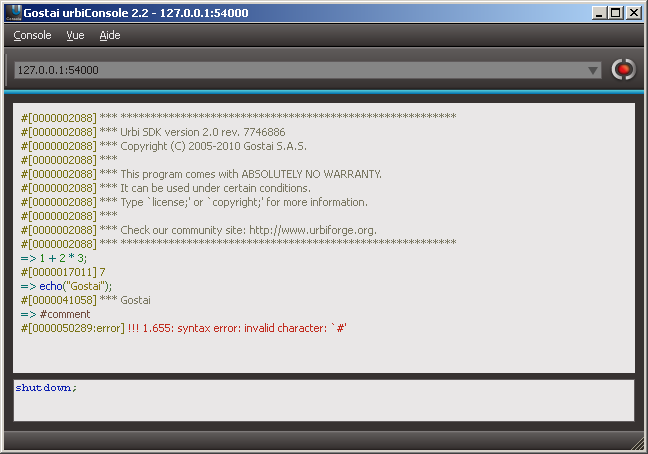
\includegraphics[width=.8\linewidth]{img/gostai-console}
  \caption{A Gostai Console session.}
  \label{fig:jazz:gostaicon}
\end{figure}

From a Windows computer, we recommend that you use Gostai Console
(\url{http://www.gostai.com/download/gostai_console/}, see
\autoref{fig:jazz:gostaicon}), a dedicated tool to connect to the Urbi
engine running on your Jazz robot.

Specify the host name and port to use (\samp{A1111FRPA001001:54000}) in the
text field in the top of the window and click on the right to start the
connection.


\subsection{Ssh Access to Jazz Filesystem}

You can use ssh to connect to Jazz and access its filesystem. If you are
using Windows you have to install Putty (\url{http://www.putty.org}). On Mac
OS X or GNU/Linux use the \lstinline{ssh} built-in client.  To connect
through ssh you have to specify in your ssh client:
\begin{itemize}
\item Jazz IP address (obtained at robot start up) or host name
\item default user login: \samp{gostai} (do not copy the quotes)
\item default user password: \samp{gostai} (do not copy the quotes)
\end{itemize}

For example, if Jazz IP address on your LAN is \samp{192.168.1.3}, then
under GNU/Linux you would have to type in a shell:

\begin{shell}
$ gostai@192.168.1.3
Login in
gostai@A1111FRPA001001:~$ # Now you are logged in Jazz, you can type shell commands
\end{shell}%$

If Jazz host name is \samp{A1111FRPA001001} and you have DNS resolution
activated in your LAN, type:

\begin{shell}
$ ssh gostai@A1111FRPA001001
Login in
gostai@A1111FRPA001001:~$ # Now you are logged in Jazz, you can type shell commands
\end{shell}%$

Once you are connected with ssh to your Jazz robot, you arrive in a Bash
shell which gives you complete access to Jazz filesystem. If you are not
familiar with GNU/Linux and the Bash shell, we advise that you read some
Bash tutorial on the Internet to familiarize with Bash basic commands.

It is not mandatory to use ssh to program your Jazz robot. It will only
becomes useful if you want to use advanced features like embedding your
code in Jazz and have it load at robot start up.

\section{Jazz internal website}
\label{sec:internalwebsite}

Jazz embed a website that allows you to configure and control it. To access this website, just enter
Jazz IP address in your browser (Internet explorer, Firefox, Chrome, ...).

\begin{figure}[!h]
  \centering
  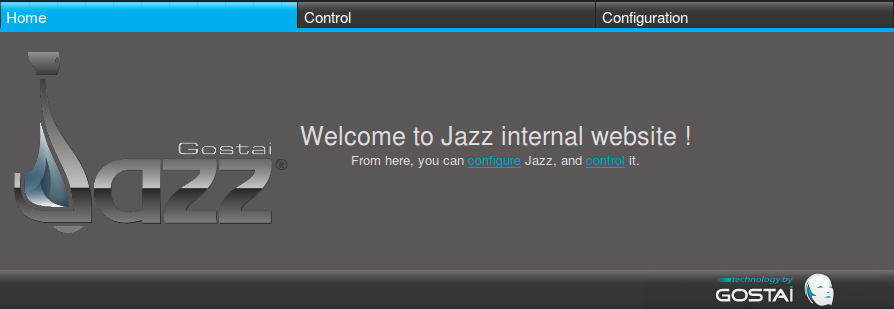
\includegraphics[width=.7\linewidth]{img/jazz/internalsite}
  \caption{Jazz Internal Website.}
  \label{fig:jazz:internalwebsite}
\end{figure}

Click on the \textit{Control} menu category to access Jazz local control
interface, or click on the \textit{Configuration} menu to access Jazz
configuration pages (WiFi, services launched, ...).

\section{Uploading and loading your code on Jazz}

\subsection{The \textit{User Services} web page}

In Jazz internal website (\autoref{sec:internalwebsite}), we provide a page
you can use to upload your own \us services to Jazz, and made it execute
them at startup. To access this page, click on the \textit{Configuration}
menu, then click on the \textit{User services} sub-menu.

\begin{figure}[!h]
  \centering
  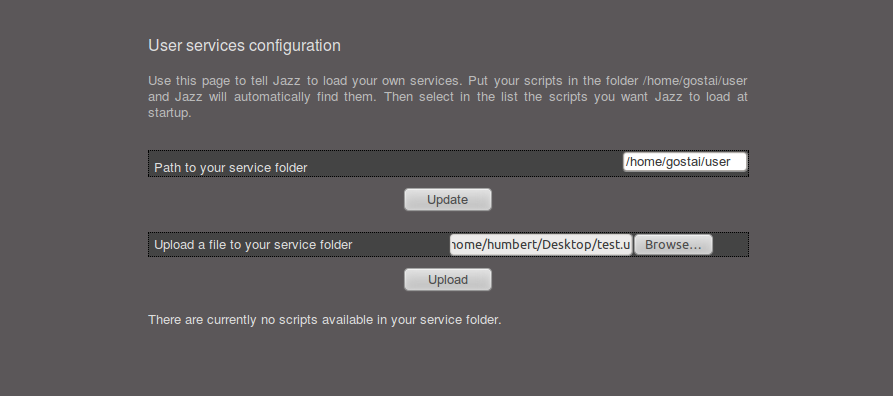
\includegraphics[width=.7\linewidth]{img/jazz/userservices1}
  \caption{User services web page.}
  \label{fig:jazz:userservice1}
\end{figure}

From this page you can change the folder where Jazz will search for your code (by default it's \lstinline{/home/gostai/user}).
To change it, edit the text field after the label \textit{Path to your service folder}, then press the \textit{Update} button below.

You can also upload \us source file to this folder. Click on the \textit{Browse} button next to the \textit{Upload a file to your service folder} label. Then choose a file on your computer. It will be automatically uploaded to the robot service folder when you press the \textit{Upload} button.
Once your file was uploaded, it will be listed on the web page.

\begin{figure}[!h]
  \centering
  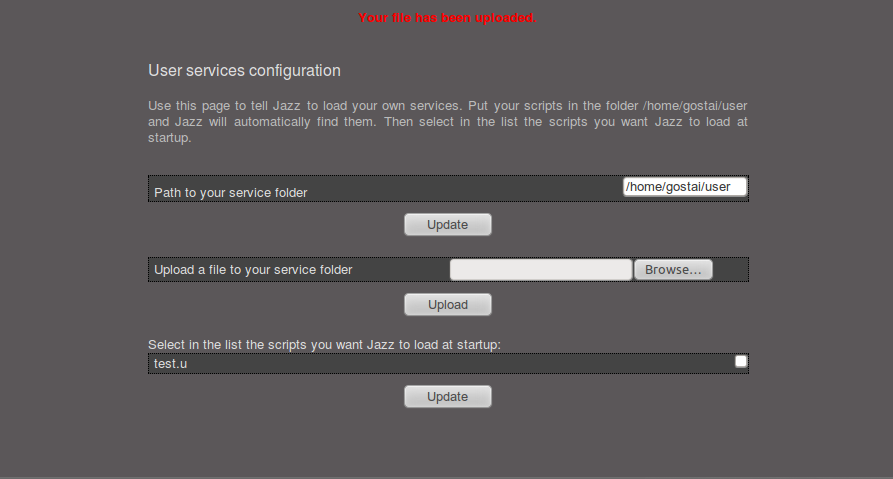
\includegraphics[width=.7\linewidth]{img/jazz/userservices2}
  \caption{User services web page: \textit{test.u} service was uploaded.}
  \label{fig:jazz:userservice2}
\end{figure}

If you want Jazz to automatically load your \us file at startup, check the check-box next to your file name, and click on the \textit{Update} button.

\begin{figure}[!h]
  \centering
  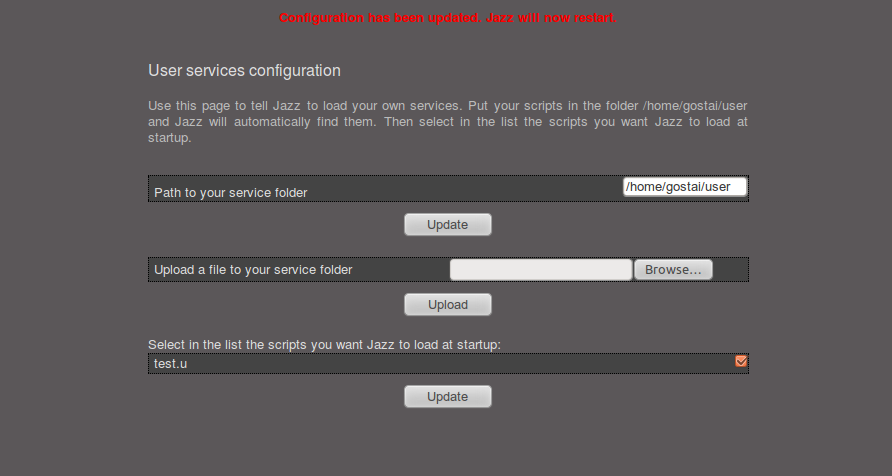
\includegraphics[width=.7\linewidth]{img/jazz/userservices3}
  \caption{User services web page: \textit{test.u} service loaded at startup.}
  \label{fig:jazz:userservice3}
\end{figure}

\subsection{Uploading Files on Jazz Filesystem using scp}

In order to upload files on Jazz filesystem you need to have a client
supporting the scp protocol.

Under GNU/Linux or similar Unix system, you can use the \command{scp}
command line tool.

\begin{shell}
$ # Copy 'myfile.u' to Jazz home folder:
$ scp myfile.u gostai@A1111FRPA001001:/home/gostai/myfile.u
\end{shell}%$

Under windows you can use WinSCP (\url{http://winscp.net/eng/docs/lang:fr})
or Pscp, the scp client that comes with Putty
(\url{http://www.chiark.greenend.org.uk/~sgtatham/putty/download.html}).

You can then verify with ssh that your file is in the robot:

\begin{shell}
$ ssh gostai@A1111FRPA001001
Login in
gostai@A1111FRPA001001:~$ ls /home/gostai/myfile.u
/home/gostai/myfile.u
\end{shell}%$

\section{Updating Jazz Software}

Gostai provides updates to Jazz software. To verify if updates are available
and automatically install them, go to Jazz internal website
(\autoref{sec:internalwebsite}), click on the \textit{Configuration} menu,
then click on the \textit{System} sub-menu.

\begin{figure}[!h]
  \centering
  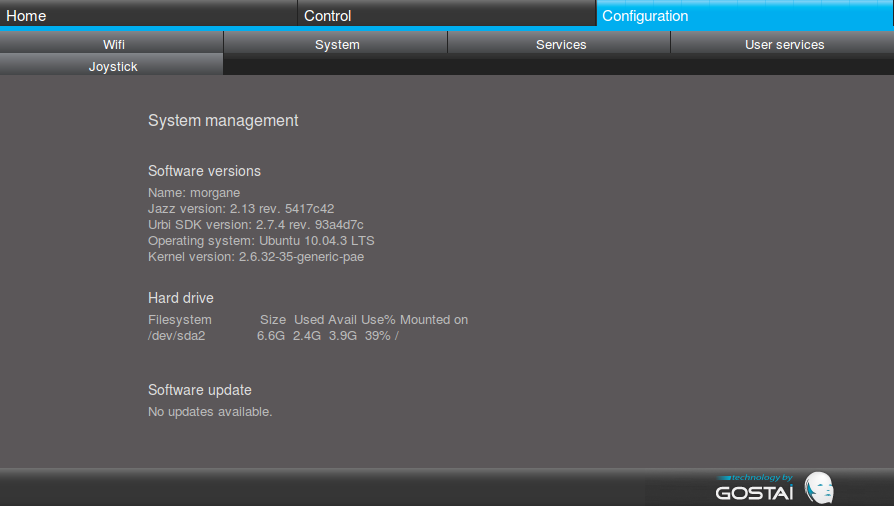
\includegraphics[width=.7\linewidth]{img/jazz/system}
  \caption{System page: display Jazz software information and allow updates.}
  \label{fig:jazz:services}
\end{figure}

Jazz will check if updates are available, and in case there are, it will
display a button that allows you to start the update process. Please do not
shutdown Jazz while updating. At the end of the update Jazz will display a
message in it's website and automatically restart.

If no updates are available, the message ``No updates available'' will be
displayed instead of the update button.

\section{Restarting Jazz Software}

To start, stop or restart Jazz software (the Urbi runtime plus Jazz Urbi
software), you can use the script \lstinline{/etc/init.d/jazz}:

\begin{shell}
gostai@A1111FRPA001001:~$ # shutdown Jazz
gostai@A1111FRPA001001:~$ /etc/init.d/jazz stop
gostai@A1111FRPA001001:~$ # start Jazz
gostai@A1111FRPA001001:~$ /etc/init.d/jazz start
gostai@A1111FRPA001001:~$ # restart Jazz
gostai@A1111FRPA001001:~$ /etc/init.d/jazz restart
\end{shell}%$

\section{Changing Software Profile}
\label{sec:jazz:profile}

The functionality described here is an advanced functionality. Do not use it
without first asking advises to Gostai. Misuse can result in Jazz
instability or breakage.

Gostai Jazz robot software is modular, and can operate with different
software profiles in function of how you want to use the robot: you can
activate all its functionalities, or only part of them.  We provide an
interface that allow to fine tune Jazz in function of your use
cases.

To access this interface go to Jazz internal web interface
(\autoref{sec:internalwebsite}), and choose the \emph{Configuration} menu,
then click on the \emph{Services} sub-menu.

You can use the shortcut button to set Jazz predefined default configuration,
or directly fine tune Jazz activating only the functionalities you
need. Please be cautious when doing so, some services have dependencies
between each other, some combinations of services might result in Jazz
instability. Always request advises from Gostai.

Press the send button when your are done to save the new configuration. Jazz
will automatically restart it's software using the new configuration.

\begin{figure}[!h]
  \centering
  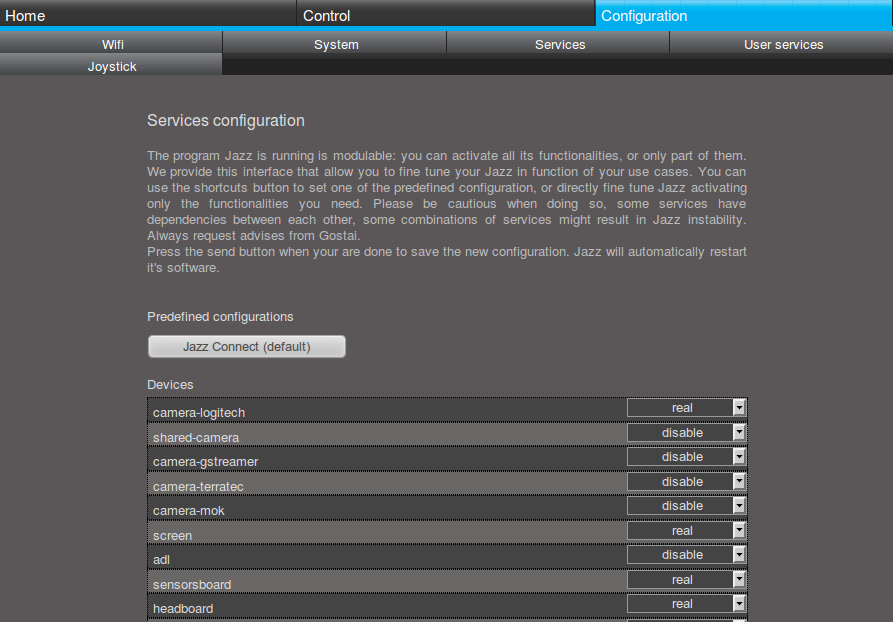
\includegraphics[width=.7\linewidth]{img/jazz/services}
  \caption{Service activation page: tune Jazz software profile.}
  \label{fig:jazz:services}
\end{figure}


\section{Using the Examples}

With the descriptions of Jazz modules API, we include \us as well as
UObjects examples to help you understand how to use the modules.

\subsection{\us Examples}

To play with \us on Jazz, you can open a telnet connection to your robot
(use netcat or Gostai Console), and copy and paste the example to evaluate
the code.

\begin{shell}[alsolanguage={[interactive]urbiscript}]
$ rlwrap nc A1111FRPA001001 54000
[00732235] *** ********************************************************
[00732235] *** Jazz version 2.10.2 rev. a2aa56e
[00732235] *** Copyright (C) 2004-2011 Gostai S.A.S.
[00732235] ***
[00732235] *** Urbi SDK version 2.7.2 rev. 7a6a48f
[00732235] *** Copyright (C) 2004-2011 Gostai S.A.S.
[00732235] ***
[00732235] *** This program comes with ABSOLUTELY NO WARRANTY.  It can
[00732235] *** be used under certain conditions.  Type `license;',
[00732235] *** `authors;', or `copyright;' for more information.
[00732235] ***
[00732235] *** Check our community site: http://www.urbiforge.org.
[00732235] *** ********************************************************
echo("hello world");
[00138887] *** hello world
\end{shell}%$

Alternatively, you can also write the \us code to a file, upload this file
on Jazz filesystem using \lstinline{scp}, and then load the code from a
telnet connection.

\begin{shell}[alsolanguage={[interactive]urbiscript}]
$ cat test.u
echo("hello world");
$ scp test.u gostai@A1111FRPA001001:/home/gostai/test.u
$ rlwrap nc A1111FRPA001001 54000
[00732235] *** ********************************************************
[00732235] *** Jazz version 2.10.2 rev. a2aa56e
[00732235] *** Copyright (C) 2004-2011 Gostai S.A.S.
[00732235] ***
[00732235] *** Urbi SDK version 2.7.2 rev. 7a6a48f
[00732235] *** Copyright (C) 2004-2011 Gostai S.A.S.
[00732235] ***
[00732235] *** This program comes with ABSOLUTELY NO WARRANTY.  It can
[00732235] *** be used under certain conditions.  Type `license;',
[00732235] *** `authors;', or `copyright;' for more information.
[00732235] ***
[00732235] *** Check our community site: http://www.urbiforge.org.
[00732235] *** ********************************************************
load("/home/gostai/test.u");
[00138887] *** hello world
\end{shell}%$

\subsection{UObjects examples}

See the \usdk documentation to know how to compile UObjects with \usdk
(using either \command{umake-shared}
(\ifthenelse{\boolean{urbisdk}}{\autoref{sec:tools:umake-shared}}{part of
  \usdk}) or Visual Studio templates).

Once you have compiled your UObject, you can run it remotely from your
computer, or embed it in the robot (you have to compile your UObject with
GNU/Linux for it to be usable on the robot).

\subsubsection{Compiling on Jazz}

Compiling on Jazz can be very slow and inconvenient, however it frees you
from the need of installing the \usdk on your computer. To compile on Jazz,
first verify that \command{umake-shared} is available in your \env{PATH}.

\begin{shell}
gostai@A1111FRPA001001:~$ which umake-shared
/usr/local/stow/urbi-sdk/bin//umake-shared
\end{shell}%$

In case \command{umake-shared} is not found, update the \env{PATH} variable.

\begin{shell}
gostai@A1111FRPA001001:~$ which umake-shared
gostai@A1111FRPA001001:~$ export PATH=/usr/local/stow/urbi-sdk/bin:$PATH
gostai@A1111FRPA001001:~$ which umake-shared
/usr/local/stow/urbi-sdk/bin//umake-shared
\end{shell}%$

Then stop Jazz runtime to free the processor for your compilation.
\begin{shell}
gostai@A1111FRPA001001:~$ /etc/init.d/jazz stop
\end{shell}%$

Upload some UObject code to your robot using \lstinline{scp}.

\begin{shell}
gostai@A1111FRPA001001:~$ cd myuob
gostai@A1111FRPA001001:~/myuob$ ls
test.cc
gostai@A1111FRPA001001:~/myuob$ cat test.cc
#include <urbi/uobject.hh>

class Test : public urbi::UObject
{
public:
  Test(const std::string& s)
    : urbi::UObject(s)
  {
    UBindFunction(Test, init);
  }

  int init()
  {
    UBindFunction(Test, foo);
    return 0;
  }

  std::string foo()
  {
    return "Hello world";
  }
};

UStart(Test);
\end{shell}%$

Now you can compile your UObjects.

\begin{shell}
gostai@A1111FRPA001001:~/myuob$ umake-shared -q -o test
gostai@A1111FRPA001001:~/myuob$ ls test.so
test.so
\end{shell}%$

You obtain a shared library containing your UObject binary code, that you
can load and use from \us.

\begin{urbiunchecked}
loadLibrary("/home/gostai/myuob/test.so");
Test;
[00711192] Test
var t = Test.new;
[00718330] Test_0xffffffffb33ab028
t.foo;
[00713182] "Hello world"
\end{urbiunchecked}

\subsubsection{Compiling on your Computer}

See the \usdk documentation to compile on your computer.  Use the same
version of \usdk that the one used in Jazz for compatibility. To get the
version of \urbi used in Jazz see \autoref{sec:troublesshoot:version}.

% FIXME plus de detail

% \section{Changing Jazz profile}
% pour passer de dev vers prod

%%% Local Variables:
%%% coding: utf-8
%%% mode: latex
%%% TeX-master: t
%%% ispell-dictionary: "american"
%%% ispell-personal-dictionary: "../urbi.dict"
%%% fill-column: 76
%%% End:
